\section{Modellering}
\subsection{Situasjon}
I den første modellen demonstrerer vi dempingen som de forskjellig frekvenskomponentene i et signal opplever når det sendes gjennom et medium. Dette gjøres ved å sende et signal med flere frekvenskomponenter gjennom en dempende funksjon, og deretter analysere hvordan de forskjellige komponentene blir påvirket.
Vi tar utgangspunkt i en firkantpuls med periode $T$:
\[
    V_{in}(t) = \begin{cases}
        5, & -\frac{T}{2} \leq t < 0 \\
        0, & 0 \leq t < \frac{T}{2} \\
    \end{cases}, \quad hvor \quad T = 2 \mu s,\qquad duty\ cycle = 50\%
\]
Vi bestemmer først Fourier-rekken til firkantpulsen for å finne frekvenskomponentene:
\[
    V_{in}(t) = c_0 + \sum_{\substack{n=-\infty\\ n\ \text{oddetall}}}^{\infty} c_n e^{j n \omega_0 t}, \quad hvor \quad \omega_0 = \frac{2\pi}{T}
\]
Merk at siden vi vet at duty cycle er 50\%, vil bare oddetalls harmoniske være tilstede i Fourier-rekken.
Koefisientene $c_n$ kan beregnes som:
\[
    c_0 = \frac{1}{T} \int_{-T/2}^{T/2} V(t) dt = \frac{5}{2}
\]
\[
    c_n = \frac{1}{T} \int_{-T/2}^{T/2} V(t) e^{-j n \omega_0 t} dt =  \frac{5}{j 2 n \pi} (1 - (-1)^n)
\]
Vi for dermed at:
\[
    V_{in}(t) = \frac{5}{2} + \sum_{\substack{n=-\infty\\ n\ \text{oddetall}}}^{\infty} \frac{5}{j n \pi} e^{j n \omega_0 t}
\]
For å modellere dempingen i mediet, antar vi parametre som gir relaistisk tilnærming til virkelige kabelverdier for R, G, L og C.
Vi antar at mediet er en Cat5e kabel med følgende parametere:
Fra formel \eqref{eq:skin-effekt} får vi at R er gitt ved:
\[
    R(f) = R_{DC} \cdot \sqrt{\frac{f}{f_{s}}}, \quad hvor \quad f_{s} = \frac{\rho_{cu}}{\pi \mu_{cu} r^2}, \quad R_{DC} = n_s \cdot \frac{\rho_{cu}}{\pi r^2}, \quad (merk\ at \quad \omega = 2\pi f)
\]
\[
    \rho_{cu} = 1.72 \cdot 10^{-8} \Omega m, \quad r = 0.255 mm, \quad \mu_{cu} = \mu_0 \cdot \mu_r = 4\pi \cdot 10^{-7} H/m., \quad n_s = 2
\]
\[
    f_s \approx 67kHz, \quad R_{DC} \approx 0.17 \Omega/m,
\]
Dermed får vi:
\[
    R(f) = 0.17 \cdot \sqrt{\frac{f}{67 \cdot 10^3}} \quad [\Omega/m]
\]
Vi antar videre at:
\[
    L = 525 nH/m, \quad C = 52 pF/m
\]
Fra formlen \eqref{eq:dielectric_loss} for dielektriske tap, får vi at:
\[
    G(f) = 2\pi f C \tan \delta, \quad hvor \quad \tan \delta = 0.002
\]
\clearpage
\noindent Vi står igjen med:
\[
    R(f) \approx 0.17 \cdot \sqrt{\frac{f}{67 \cdot 10^3}} \quad [\Omega/m], \quad L = 525 nH/m, \quad C = 52 pF/m, \quad G(f) \approx 0.65f \quad [pS/m]
\]

\noindent Vi har nå alt vi trenger for å finne overføringsfunksjonen til mediet:
\[
    H(f, l) = e^{-\gamma(f) l}, \quad hvor \quad \gamma(f) = \sqrt{(R(f) + j 2\pi f L)(G(f) + j 2\pi f C)}
\]
Her er $l$ lengden på mediet (kabelen) og $\gamma(f)$ er propagasjonskonstanten som avhenger av frekvensen.
Vi kan nå finne ut hvordan hver frekvenskomponent i firkantpulsen blir dempet ved å multiplisere hver komponent med $H(f, l)$:
\[
    V_{out}(t) = c_0H(0, l) + \sum_{\substack{n=-\infty\\ n\ \text{oddetall}}}^{\infty} c_n H(n f_0, l) e^{j n \omega_0 t}
\]
Som i hvor situasjon gir:
\[
    V_{out}(t) = \frac{5}{2}H(0, l) + \sum_{\substack{n=-\infty\\ n\ \text{oddetall}}}^{\infty} \frac{5}{j n \pi} H(n f_0, l) e^{j n \omega_0 t}    
\]
For å simulere dette numerisk, kan vi bruke Python til å beregne $H(f, l)$ for en rekke frekvenser og deretter rekonstruere tidsdomenesignalet ved hjelp av den inverse Fourier-transformasjonen.
Vi kan da plotte både inngangssignalet og utgangssignalet for å visualisere effekten av dempingen i mediet.
\clearpage
\subsection{Modeller}
For å forstå hvordan forskjellige aspekter av mediets egenskaper påvirker signalet, har vi laget flere modeller der vi varierer hvilke deler av den propagasjonskonstanten $\gamma(f)$ vi tar hensyn til. Modellene er basert på 10m, 50m, 100m og 1000m. Vi har følgende modeller:
\begin{itemize}
    \item \textbf{Kun demping:} I disse modellene tar vi kun hensyn til dempingen i mediet, og ignorerer faseendringen. Dette viser hvordan signalets amplitude påvirkes uten å endre dets form (modell 1 og 2).
    \[
        \gamma(f) = \alpha(f)
    \]
    \item \textbf{Kun faseendring:} I denne modellen tar vi kun hensyn til faseendringen i mediet, og ignorerer dempingen. Dette viser hvordan signalet ville oppføre seg i et ideelt tapsfritt medium (modell 3).
    \[
        \gamma(f) = j\beta(f)
    \]
    \item \textbf{Ideell, tapsfri og ikke-dispersiv modell:} Her antar vi at mediet er ideelt, uten demping og uten dispersjon. Dette betyr at alle frekvenskomponenter har samme fasehastighet (modell 4).
    \[
        \gamma(f) = j\beta(f), \quad hvor \quad \beta(f) = \omega\sqrt{LC}
    \]
    \item \textbf{Full modell:} Her tar vi hensyn til både demping (Re($\gamma$)) og faseendring (Im($\gamma$)) i mediet. Dette gir en tilnærmet representasjon av hvordan signalet påvirkes (modell 5).
    \[
        \gamma(f) = \alpha(f) + j\beta(f)
    \]
    \item \textbf{Waterfall plott:} For å visualisere hvordan forskjellige frekvenskomponenter påvirker tidsdomenesignalet, har vi laget to "waterfall" plot som viser hvordan signalet endres når vi inkluderer flere og flere frekvenskomponenter opp til en viss grensefrekvens (modell 6).
\end{itemize}
\clearpage
\subsection{Modell 1 (kun demping i frekvensdomenet)}
Demping av signalet er vist i figur \ref{fig:modell1}. Vi ser at høyfrekvente komponenter blir betydelig dempet, noe som resulterer i en mer avrundet firkantpuls ved utgangen. Dette illustrerer hvordan mediet fungerer som et lavpassfilter, hvor de høyere frekvensene reduseres mer enn de lavere frekvensene.
\begin{figure}[h]
    \centering
    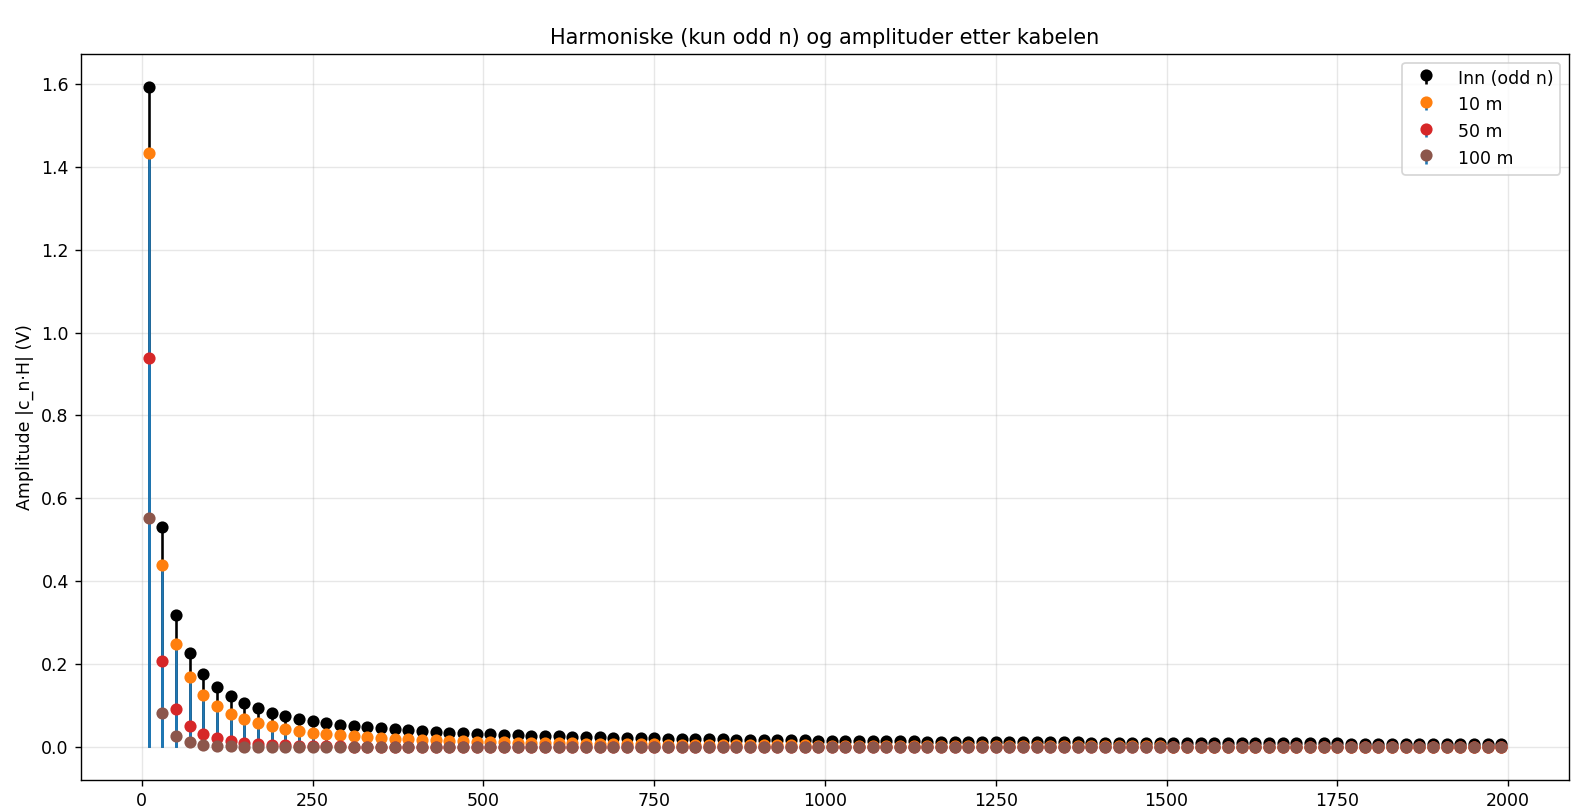
\includegraphics[width=1\textwidth]{Media/modellering1.png}
    \caption{Frekvensdomeneanalyse av firkantpuls etter å ha passert gjennom et dempende medium over forskjellige lengder.}
    \label{fig:modell1}
\end{figure}
\clearpage
\subsection{Modell 2 (demping i frekvensdomenet i tidsdomenet)}
I den andre modellen ser vi på hvordan tidsdomenesignalet endres etter å ha passert gjennom mediet. Vi rekonstruerer tidsdomenesignalet ved å summere Fourier-rekkene for de dempede harmoniske. Her har vi kun tatt hensyn til amplitudendringen, og ikke faseendringen. Altså ser vi på:
\[
    H(f, l) = e^{-\alpha(f) l}, \quad hvor \quad \alpha(f) = Re(\gamma(f))
\]
Resultatet er vist i figur \ref{fig:modell2}. Vi ser at firkantpulsen blir mer avrundet etter å ha passert gjennom mediet, noe som bekrefter at høyfrekvente komponenter dempes mer enn lavfrekvente komponenter. Dette resulterer i en signifikant endring i signalets form, spesielt over lengre avstander.
\begin{figure}[h]
    \centering
    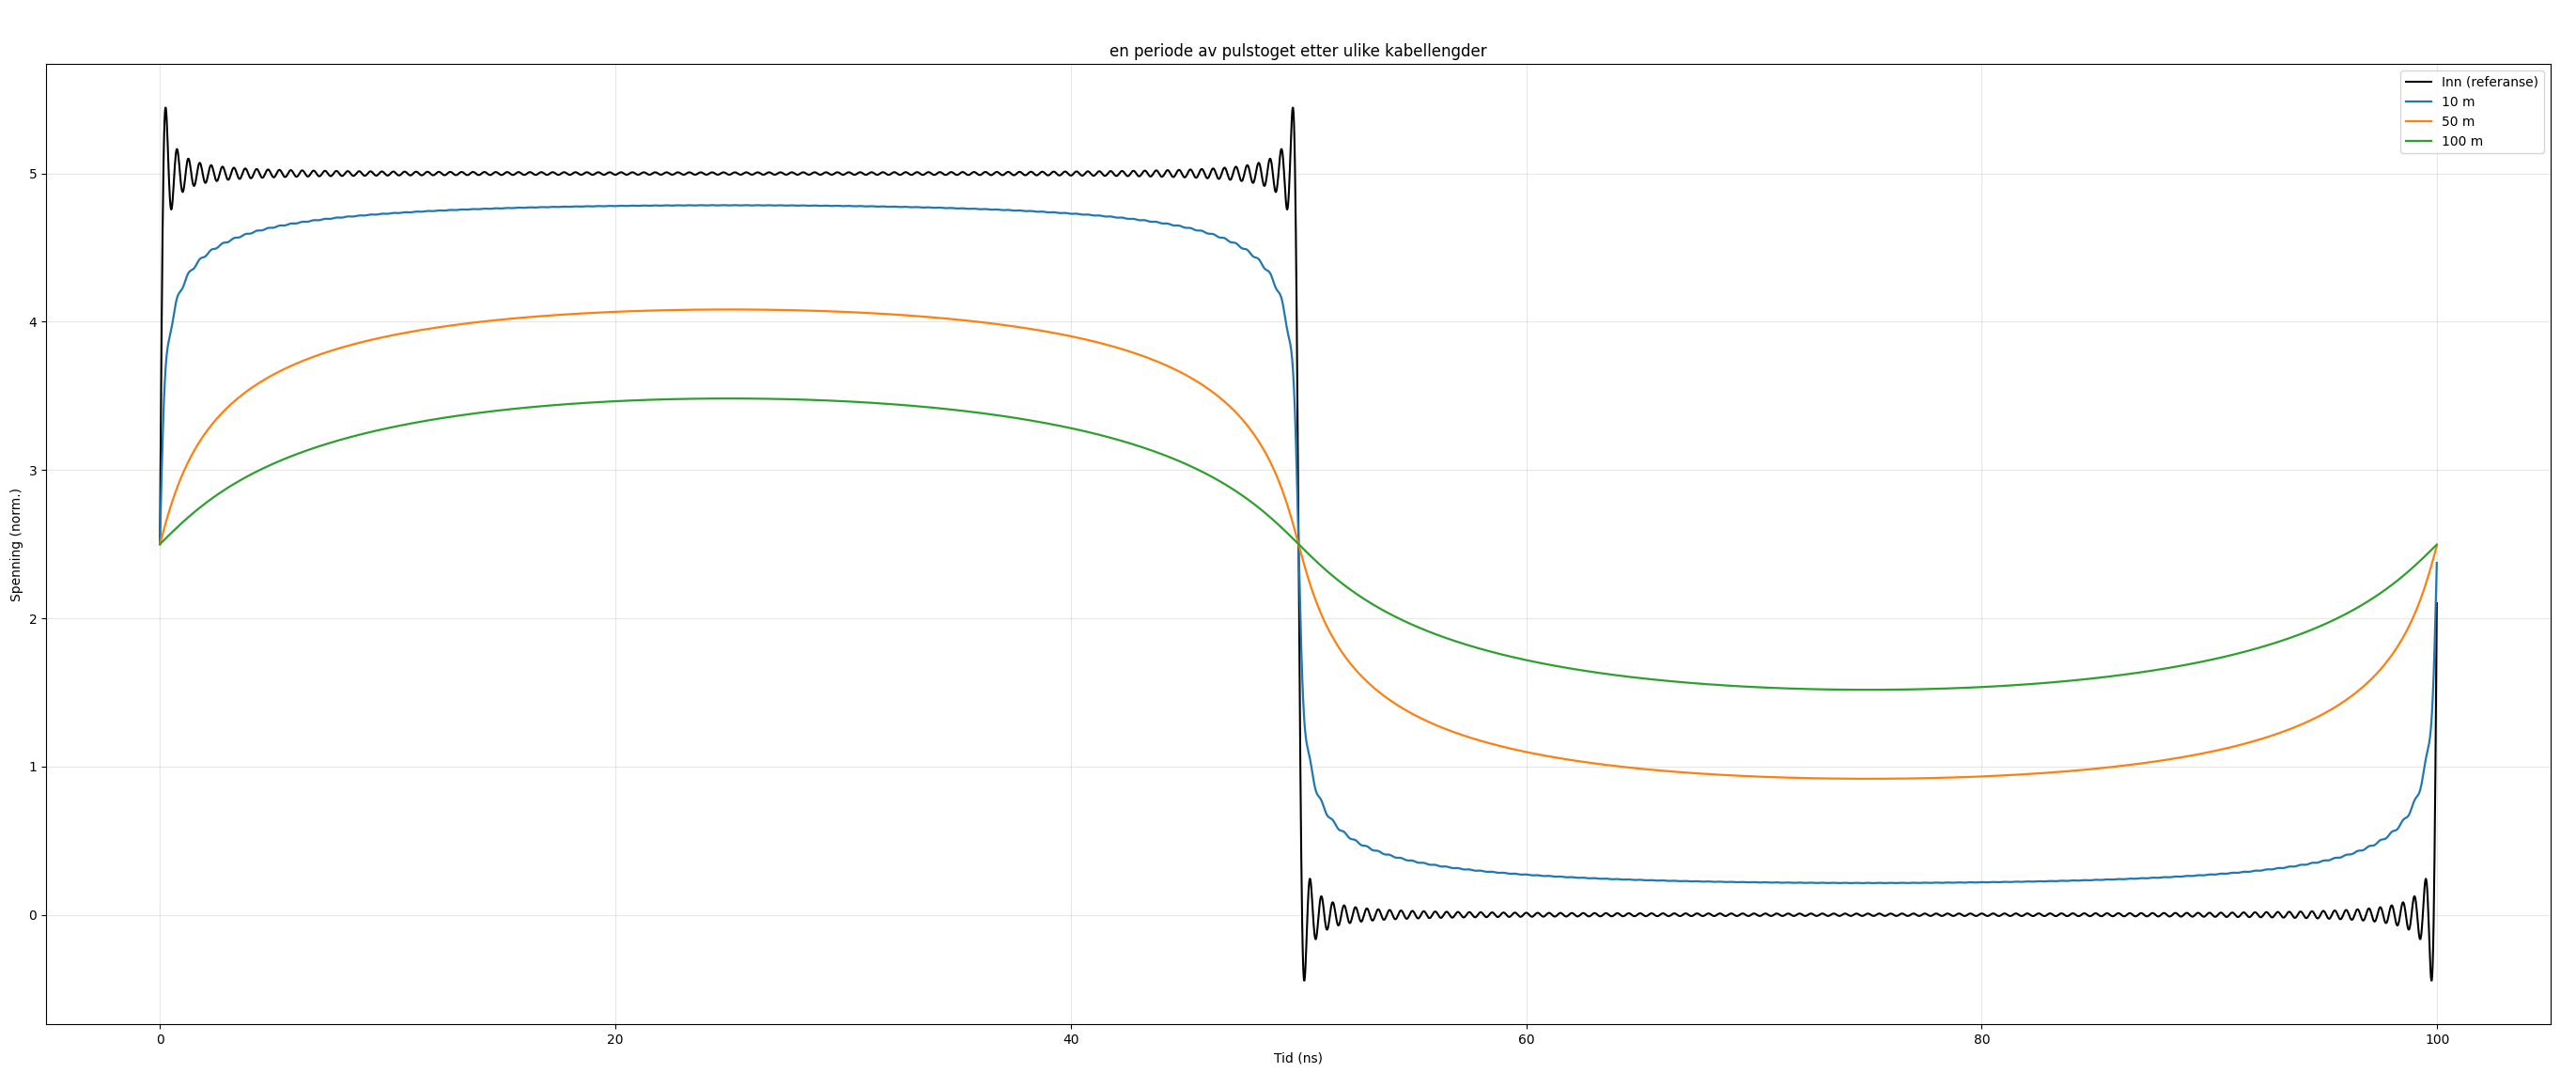
\includegraphics[width=1\textwidth]{Media/modellering2.png}
    \caption{Tidsdomenesignalet av firkantpuls etter å ha passert gjennom et dempende medium over forskjellige lengder.}
    \label{fig:modell2}
\end{figure}
\clearpage
\subsection{Modell 3 (kun faseendring)}
I den tredje modellen ser vi på hvordan tidsdomenesignalet endres når vi kun tar hensyn til faseendringen i mediet, og ignorerer dempingen. Altså ser vi på:
\[
    H(f, l) = e^{-j\beta(f) l}, \quad hvor \quad \beta(f) = Im(\gamma(f))
\]
Resultatet er vist i figur \ref{fig:modell3}. Vi ser at firkantpulsen blir mer vrengete etter å ha passert gjennom mediet, men beholder sin generelle form. Dette illustrerer hvordan faseendringen påvirker signalets tidsdomenesignal uten å endre dets amplitude. Alle frekvenskomponenter opplever forskjellige faseforsinkelser, noe som fører til en forvrengning av signalets form.
\begin{figure}[h]
    \centering
    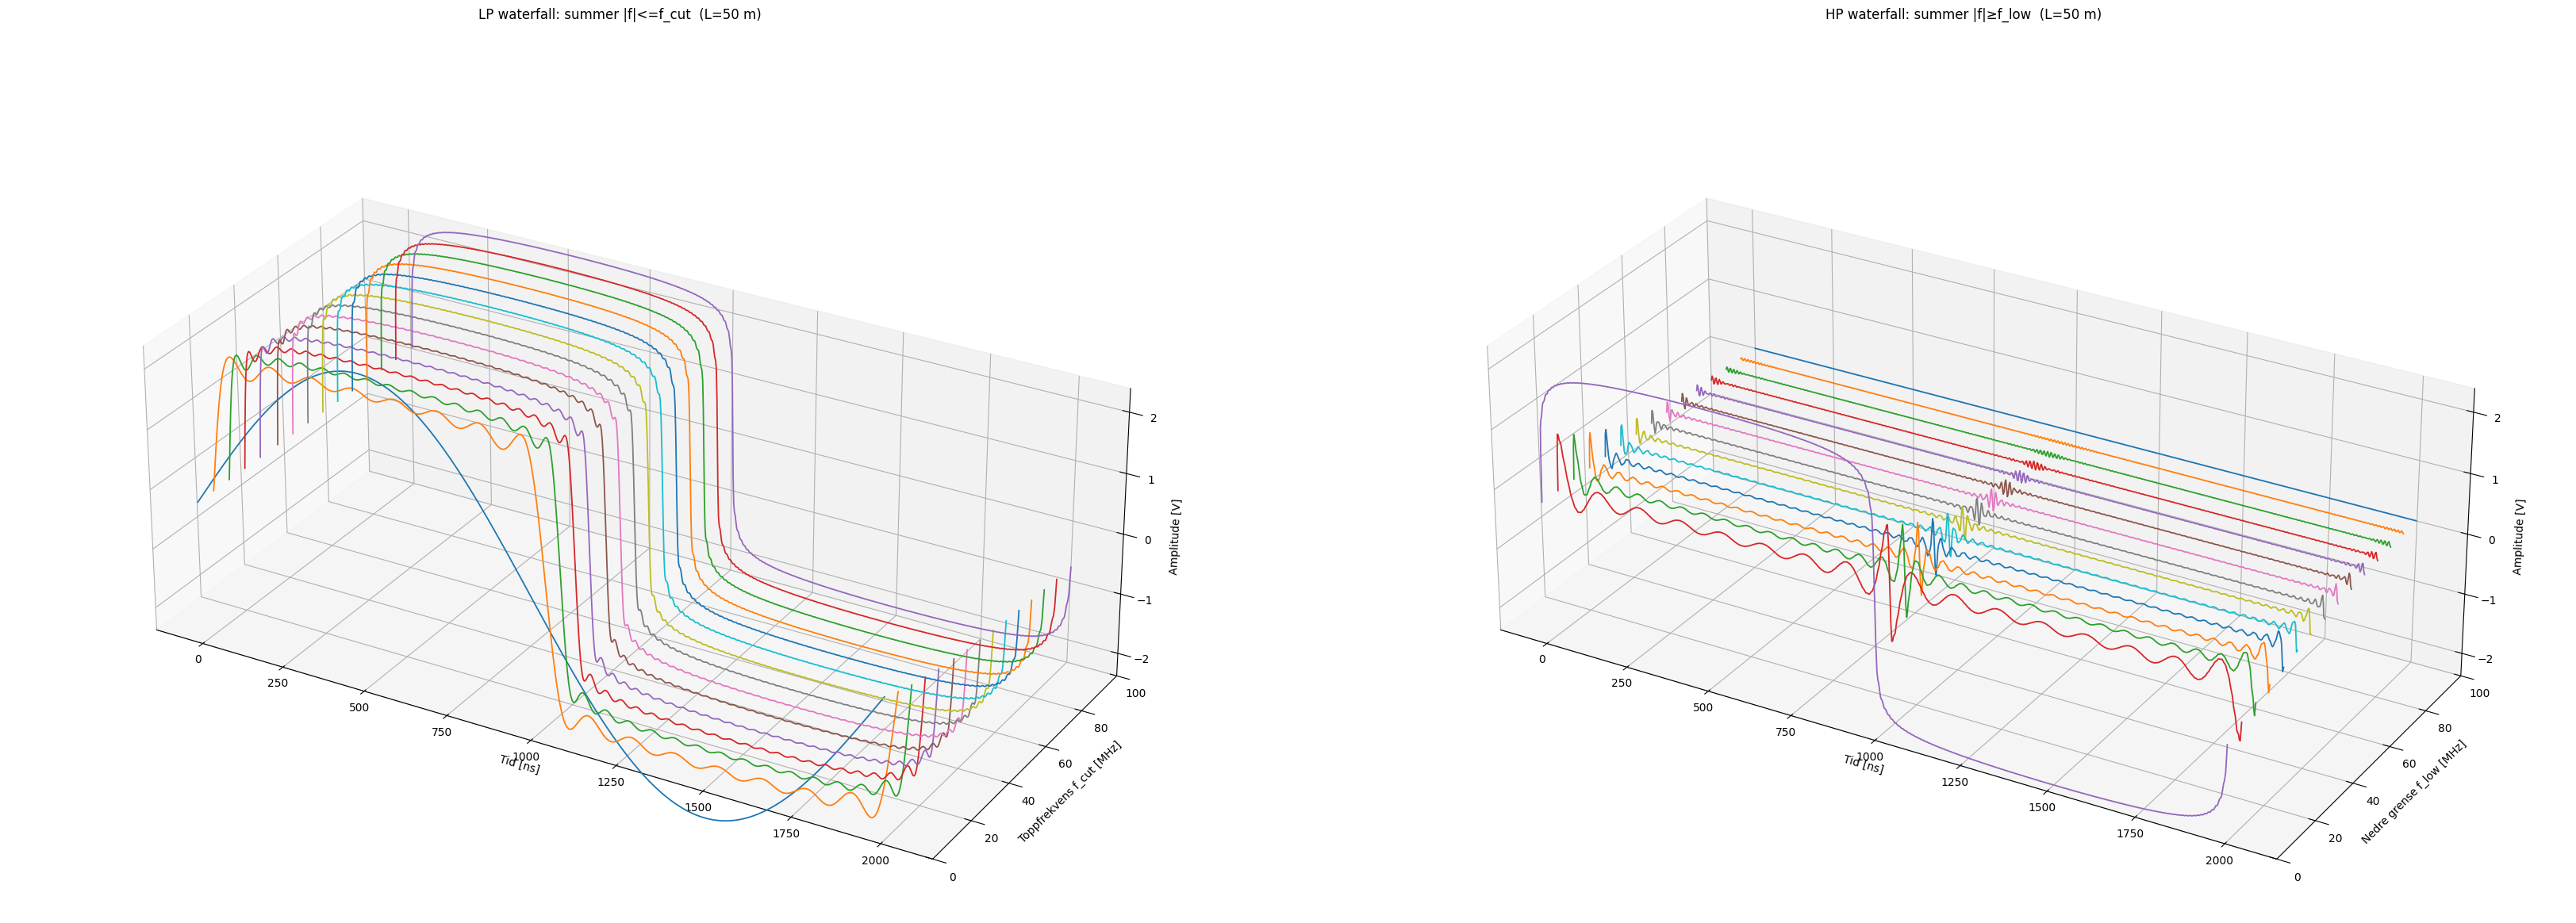
\includegraphics[width=1\textwidth]{Media/modellering3.png}
    \caption{Tidsdomenesignalet av firkantpuls etter å ha passert gjennom et medium med kun faseendring.}
    \label{fig:modell3}
\end{figure}
\clearpage
\subsection{Modell 4 (Ideell, ikke-dispersiv modell)}
I den fjerde modellen ser vi på hvordan tidsdomenesignalet endres når vi antar at mediet er ideelt, uten demping og uten dispersjon. Altså ser vi på:
\[
    H(f, l) = e^{-j\beta(f) l}, \quad hvor \quad \beta(f) = \omega\sqrt{LC}
\]
Resultatet er vist i figur \ref{fig:modell4}. Vi ser at firkant
pulsen opprettholder sin opprinnelige form og blir forsinket i tid. Dette bekrefter at i et ideelt ikke-dispersivt medium, har alle frekvenskomponenter samme fasehastighet, noe som betyr at signalets form bevares uten noen forvrengning.
\begin{figure}[h]
    \centering
    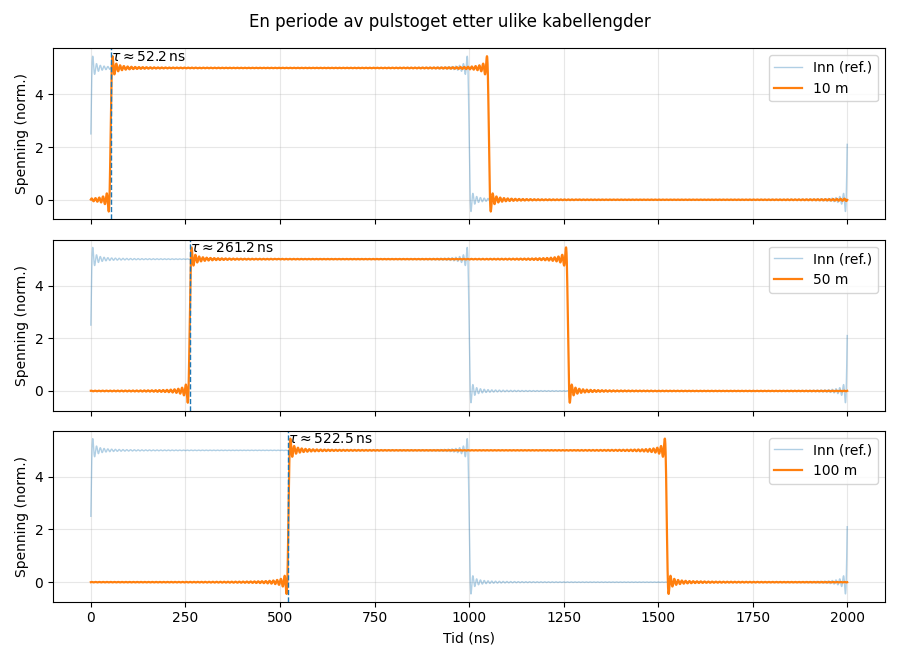
\includegraphics[width=1\textwidth]{Media/modellering4.png}
    \caption{Tidsdomenesignalet av firkantpuls etter å ha passert gjennom et ideelt ikke-dispersivt medium over forskjellige lengder.}
    \label{fig:modell4}
\end{figure}
\clearpage
\subsection{Modell 5 (full modell)}
I den femte modellen ser vi på hvordan tidsdomenesignalet endres når vi tar hensyn til både demping og faseendring i mediet. Altså ser vi på:
\[
    H(f, l) = e^{-\gamma(f) l}, \quad hvor \quad \gamma(f) = \alpha(f) + j\beta(f)
\]
Resultatet er vist i figur \ref{fig:modell5}. Vi ser at firkantpulsen blir både dempet og forsinket i tid etter å ha passert gjennom mediet. Dette gir en mer realistisk representasjon av hvordan signalet påvirkes i et ekte medium, hvor både demping og faseendring spiller en rolle. Over lengre avstander blir signalet stadig mer forvrengt, noe som illustrerer viktigheten av å ta hensyn til begge aspekter for å forstå signalets oppførsel.
\begin{figure}[h]
    \centering
    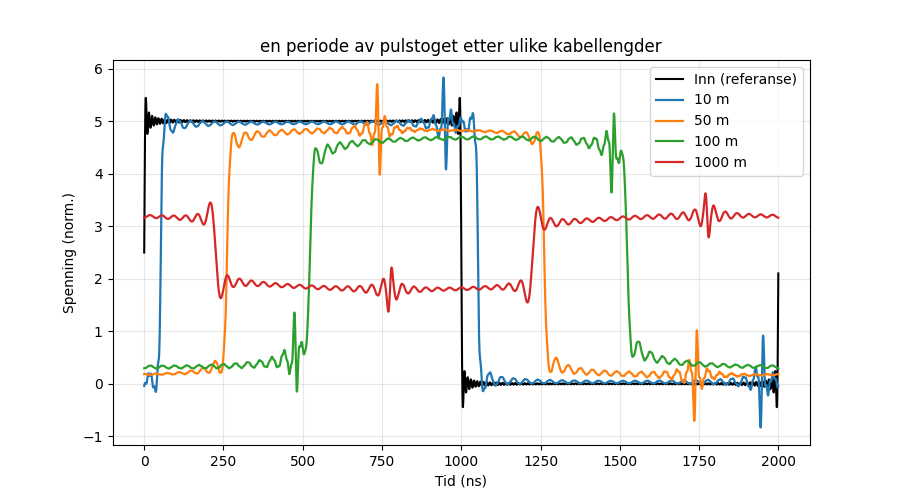
\includegraphics[width=1\textwidth]{Media/modellering5.png}
    \caption{Tidsdomenesignalet av firkantpuls etter å ha passert gjennom et realistisk medium over forskjellige lengder.}
    \label{fig:modell5}
\end{figure}
\clearpage
\subsection{Modell 6 (waterfall plot)}
For å få en bedre forståelse av hvordan forskjellige frekvenskomponenter påvirker tidsdomenesignalet, har vi laget to "waterfall" plot som viser hvordan signalet endres når vi inkluderer flere og flere frekvenskomponenter opp til en viss grensefrekvens (Visualisere bidraget fra hver komponent). Den ene kalles lavpassfilter (LP) og den andre høypassfilter (HP). Prinsippet er det samme for begge plottene, men de summerer forskjellige sett av frekvenskomponenter:
\begin{itemize}
    \item \textbf{Lavpassfilter (LP):} Her summerer vi alle frekvenskomponenter fra fundamentalfrekvensen $f_0$ opp til en økende grensefrekvens $f_{cut}$. Dette viser hvordan tidsdomenesignalet utvikler seg når vi inkluderer flere lavfrekvente komponenter.
    \[
        |f| \leq f_{cut}
    \]
    \item \textbf{Høypassfilter (HP):} Her summerer vi alle frekvenskomponenter fra en synkende grensefrekvens $f_{low}$ opp til en øvre grensefrekvens (for eksempel 100 MHz eller høyeste harmoniske). Dette viser hvordan tidsdomenesignalet påvirkes når vi inkluderer flere høyfrekvente komponenter.
    \[
        |f| \geq f_{low}
    \]
    \item \textbf{Antall kutt:} For å få en jevnere overgang i waterfall plottene, har vi økt antall kutt (cuts) til 15. Dette gir en mer detaljert visualisering av hvordan signalet endres med forskjellige grensefrekvenser.
\end{itemize}
Dette er vist i figur \ref{fig:modell6}.
\begin{figure}[h]
    \centering
    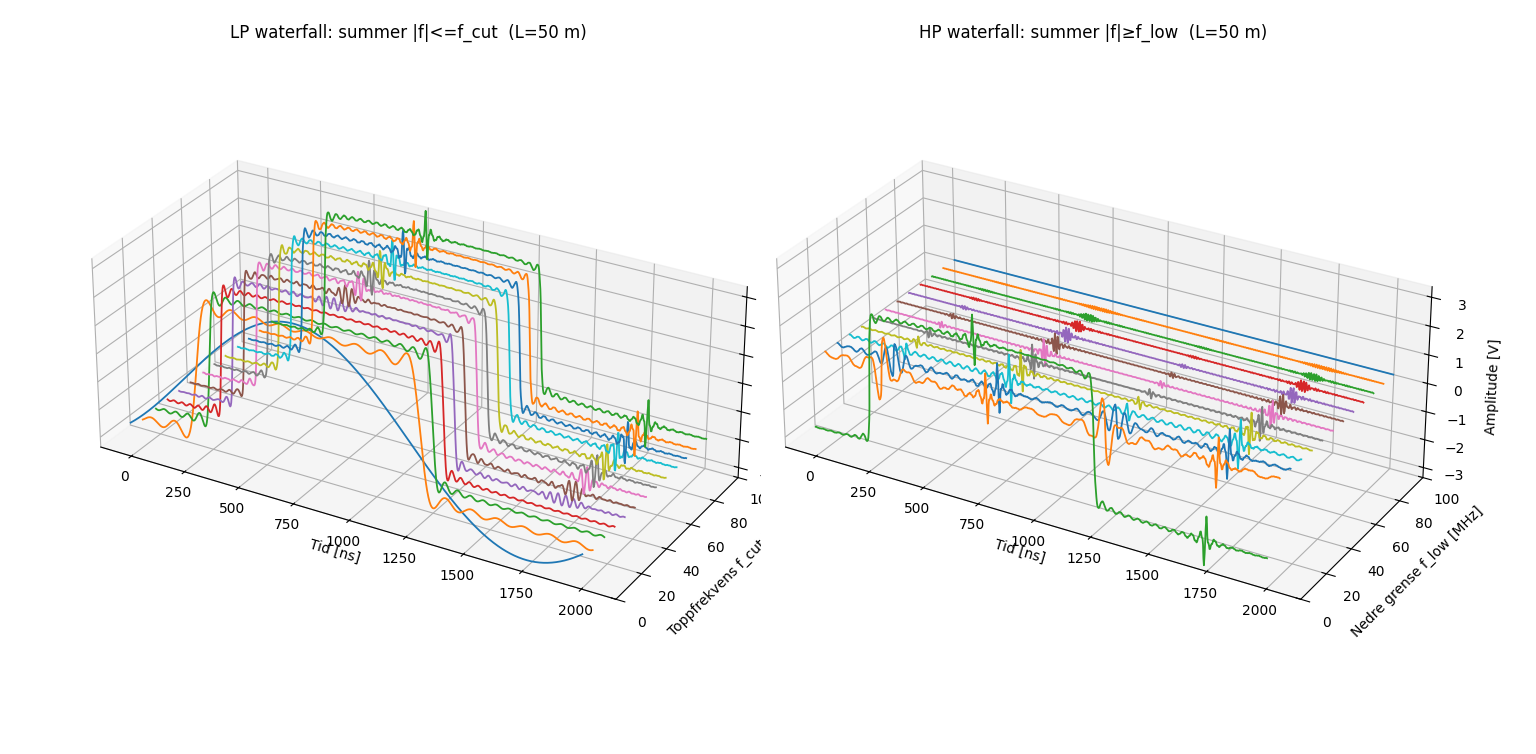
\includegraphics[width=1\textwidth]{Media/modellering6.png}
    \caption{Waterfall plot som viser hvordan tidsdomenesignalet endres når flere frekvenskomponenter inkluderes opp/ned til forskjellige grensefrekvenser (plottet er for 50m kabel).}
    \label{fig:modell6}
\end{figure}\\
Vi ser at når vi inkluderer flere frekvenskomponenter, blir tidsdomenesignalet mer detaljert og nærmere den opprinnelige firkantpulsen. Dette illustrerer viktigheten av høyfrekvente komponenter for å bevare signalets form. For lavpassfilteret ser vi at signalet gradvis nærmer seg firkantpulsen når flere lavfrekvente komponenter inkluderes. For høypassfilteret ser vi at signalet blir mer avrundet når flere høyfrekvente komponenter inkluderes, noe som bekrefter at høyfrekvente komponenter er avgjørende for å opprettholde skarpe overganger i tidsdomenesignalet.
\clearpage

